\chapter{2D grafika: knižnica SDL}
\label{sect:SDL}

Doteraz všetky naše programy čítali vstup zo štandardného vstupu  (\vb{cin}) a
vypisovali na štandardný výstup (\vb{cout}), prípadne do súboru.  V tejto časti
bude našim hlavným cieľom naučiť sa písať programy, ktoré pracujú s grafikou, a
dať nášmu programu na \btr pekné grafické prostredie.

Na úvod zlá správa: C++ nemá v štandardných knižniciach žiadne funkcie na prácu
s grafikou.  Nie je to tým, že by vývojári na to zabudli, je to zámer: C++ sa
používa v rôznych zariadeniach, od chladničiek po datacentrá, takže si ťažko
predstaviť rozumnú sadu funkcií, ktorá by všetkých uspokojila.

Programovanie grafiky je preto plné krvavých detailov: sú rôzne operačné
systémy, rôzne grafické systémy, rôzny hardvér, a pre každú kombináciu to treba
robiť jemne inak. Dobrá správa je, že existujú knižnice, ktoré špinavú robotu
urobia za nás.  Tento tutoriál sa snaží byť ``self-contained'', to znamená, že
okrem kompilátora, štandardných knižníc (a programu \vb{make}) nepoužívame
žiadne externé knižnice. Teraz ale urobíme výnimku a predstavíme si knižnicu
\link{https://www.libsdl.org/}{Simple DirectMedia Layer} (SDL).  Aj keď nie je
súčasťou štandardu, je veľmi rozšírená a dá sa nainštalovať úplne všade. Zároveň je {\em open source},
takže si napr. na \link{https://github.com/libsdl-org/SDL}{GitHube} môžeš pozrieť ako je naprogramovaná.
Zlá
správa je, že SDL je napísaná v jazyku C a nie C++. Dobrá správa je, že nám to
nijak nevadí: v C++ ju môžeš normálne používať.  Najprv ale: čo je to knižnica? \indexItem{Prg}{knižnica} 

Z kapitoly \ref{sect:makefile} vieš, ako skompilovať program po častiach: najprv sa urobí object code v súboroch \vb{.o} a tie sa potom
zlinkujú do výsledného programu (na to musí linker nájsť práve jednu funkciu, ktorá sa volá \vb{main}, a tá sa spustí ako prvá v programe).
Ak nemáš funkciu \vb{main}, stále môžeš vyrobiť object code, ale nedá sa z neho vytvoriť spustiteľný súbor. Viacero object code súborov sa
ale dá zabaliť do špeciálneho archívu, ktorý sa volá knižnica. Tá sa potom dá jedným príkazom pridať linkeru. Knižnica SDL je rozdelená na viacero
častí (na font, zvuk, bitmapy a pod.). Na to, aby si ich mohol používať, ich treba mať nainštalované. Ako to presne spraviť, záleží od operačného systému,
napr. v linuxových distribúciách ako Debian, Ubuntu a pod. sa dá napísať \vb{sudo apt-get install libsdl2-dev}. Tým sa jednak nakopíruje knižnica 
do nejakého štandardného adresára, kam sa kompilátor pozerá (napr. \vb{/usr/lib/x86\_64-linux-gnu/libSDL2.so}) a jednak sa nakopírujú súbory \vb{.h}
s deklaráciami do nejakého iného štandardného adresára (napr. \vb{/usr/include/SDL2}).

Ak máš knižnicu SDL nainštalovanú, môžeš použiť  \link{\rootpath/sdl/01/Makefile}{Makefile} z kapitoly~\ref{sect:makefile} a v linkovacom príkaze pre hlavný súbor pridať

\begin{Verbatim}[frame=single]
main: $(objects)
  mkdir -p $(builddir)
  g++ -O3 -std=c++20 $(objects) -o $@ \textcolor{orange}{-lSDL2}
\end{Verbatim}

Tým hovoríš linkeru, že okrem tvojich object code súborov \vb{\$(objects)} má brať do úvahy aj tie, ktoré nájde v súbore \vb{libSDL2.so}. Teraz otestujeme, či všetko funguje.
Napíš si tento program \link{\rootpath/sdl/01/main.cc}{main.cc}\\

\begin{lstlisting}[label={l:sdl.1}]
#include <SDL2/SDL.h> @\ll1@

SDL_Window* window = nullptr; @\ll4@
SDL_Renderer* renderer = nullptr;

int main() {
  SDL_Init(SDL_INIT_VIDEO | SDL_INIT_TIMER | SDL_INIT_AUDIO); @\ll2@

  window = SDL_CreateWindow("prvy pokus", SDL_WINDOWPOS_CENTERED, @\ll5@
                            SDL_WINDOWPOS_CENTERED, 800, 600,
                            SDL_WINDOW_RESIZABLE | SDL_WINDOW_SHOWN);
  renderer = SDL_CreateRenderer(window, -1, SDL_RENDERER_ACCELERATED); @\ll7@

  SDL_SetRenderDrawColor(renderer, 250, 180, 0, 255);@\ll8@   // nastav žltú farbu 
  SDL_RenderClear(renderer);@\ll9@                            // vyfarbi celú plochu 

  SDL_Rect r{.x=300,.y=200,.w=200,.h=200};@\ll{10}@              // obdĺžnik v strede okna  
  SDL_SetRenderDrawColor(renderer, 20, 30, 180, 255);@\ll{11}@   // nastav modrú farbu 
  SDL_RenderFillRect(renderer, &r);@\ll{12}@                     // vyplň obdĺžnik

  SDL_RenderPresent(renderer);@\ll{13}@                          // zobraz nakreslené veci

  SDL_Delay(2000);                                      // 2s čakaj

  SDL_DestroyWindow(window); @\ll6@
  SDL_Quit(); @\ll3@
}
\end{lstlisting}

a spusti \vb{make}. Mal by sa ti vyrobiť súbor \vb{main}, ktorý keď spustíš, otvorí sa žlté okno s modrým štvorcom 
a po dvoch sekundách zmizne. Ak sa ti to podarilo, môžeme pokračovať
a pozrieť sa, ako je SDL urobená. Je v nej dosť vecí, tu ti ukážem iba základných zopár, ktoré budeme potrebovať. Zoznam všetkých funkcií nájdeš
na \link{https://wiki.libsdl.org/SDL2}{SDL2 wiki} v časti \vb{API reference}.

Prvá vec je celkový dizajn. Keďže SDL je písaná v jazyku C, nemá konštruktory, deštruktory, ani metódy (iba typy a ``obyčajné'' funkcie),
preto dizajnéri SDL ich simulujú ``ručne''.
Jednoduchý príklad: keby si chcel mať spievajúcu uhorku, v C++ si spravíš typ, s ktorým sa bude pracovať asi takto:

\begin{lstlisting}
Uhorka* uh = new Uhorka("Chuck");   // volá sa konštruktor
uh->spievaj(42);                    // metóda
delete uh;                          // volá sa deštruktor
\end{lstlisting}

Alebo takto:

\begin{lstlisting}
{
  Uhorka uh("Chuck");  // volá sa konštruktor
  uh.spievaj(42);      // metóda
}  // tu sa tiež volá deštruktor
\end{lstlisting}

V SDL (ako v skoro každej Cčkovskej knižnici) by to bolo urobené nejak takto:

\begin{lstlisting}
Uhorka* uh = SDL_VyrobUhorku("Chuck");  // ``konštruktor'' alokuje pamäť a vráti pointer
SDL_UhorkaSpievaj(uh, 42);  // *this sa pošle ručne
SDL_ZmazUhorku(uh);         // ``deštruktor''  uvoľní pamäť
\end{lstlisting}

Poďme si rozobrať náš \vb{main.cc}. Najprv treba (riadok~\ref{l:sdl.1-1}) vložiť deklarácie zo
\prg!SDL2/SDL.h!. Pred prvým volaním nejakej funkcie treba celú knižnicu zapnúť (riadok~\ref{l:sdl.1-2}) volaním
\prg!SDL_Init(...)!; parameter udáva, ktoré časti sa majú inicializovať\footnote{
  To \prg!SDL_INIT_VIDEO!, \prg!SDL_INIT_TIMER!  atď. sú konštanty, ktoré sú postupne mocniny 2,
  preto v dvojkovej sústave každému zodpovedá jeden bit. Takže keď ich spojíš
  pomocou bitového OR, dostaneš číslo, v ktorom o každom subsytéme zistíš, či ho treba zapnúť,
  tak, že skontroluješ príslušný bit. Toto je technika, ktorá sa často používa na to, aby
  si mal sadu prepínačov v jednom čísle.
}. Pred skončením programu je slušné celú knižnicu vypnúť (riadok~\ref{l:sdl.1-3}).

Prvým typom, ktorý treba použiť,\indexItem{Prg}{\vb{SDL\_Window}, \vb{SDL\_Renderer} a vykresľovacie funkcie} 
je \vb{SDL\_Window}, v ktorom sú všetky premenné potrebné na spravovanie okna na obrazovke. Podobne ako väčšina typov v SDL, je
\vb{SDL\_Window} tzv. {\em opaque} typ: nikdy nebudeme potrebovať pristupovať k jeho premenným, vždy ho iba pošleme ako parameter do príslušných funkcií.
Hneď na začiatku na riadku~\ref{l:sdl.1-4} si spravíme globálnu premennú \prg!SDL_Window *window!. Prvá vec, ktorú po zapnutí knižnice urobíme, je 
vyrobenie okna. Na riadku \ref{l:sdl.1-5} zavoláme ``koštruktor'', ktorý vyrobí okno\footnote{Parametre sú v poradí názov, pozícia na obrazovke ($x,y$),
rozmery (šírka$\times$výška) a nastavenia; ich
presný popis je na \dlink{https://wiki.libsdl.org/SDL2/SDL_CreateWindow}, nateraz nám stačia tieto.}. V tomto momente sa na obrazovke objaví prázdne okno. Po skončení práce okno zavrieme
volaním ``deštruktora'' na riadku~\ref{l:sdl.1-6}.

Zobrazovacie funkcie nepracujú priamo s oknom, ale s premennou typu \vb{SDL\_Renderer}\footnote{Renderer je oddelený od okna kvôli tomu, že niekedy chceš 
kresliť veci nie priamo do okna, ale do poľa v pamäti
a to potom ich uložiť do súboru ako obrázok, 
alebo použiť ako textúru (napr. ak v 3D hre chceš mať zrkadlo). \vb{SDL\_CreateSoftwareRenderer} vyrobí renderer, ktorý namiesto okna používa pole v pamäti,
takže na kreslenie potom môžeš používať rovnaké funkcie: renderer ako renderer.}. Na riadku~\ref{l:sdl.1-7} vyrobíme renderer, ktorý bude kresliť do okna \vb{window}.
V SDL má ľavý horný roh okna súradnice $(0,0)$, $x$-ová súradnica ide smerom doprava, $y$-ová smerom dole a všetky sú celočíselné (t.j. pixely).

V nasledujúcich riadkoch ideme konečne kresliť: na riadku~\ref{l:sdl.1-8} rendereru povieme, aby použil tmavožltú farbu (parametre sú RGBA zložky) 
a následne na riadku~\ref{l:sdl.1-9} aby prekreslil celé pozadie. 

Na riadku~\ref{l:sdl.1-10} vyrobíme premennú typu \vb{SDL\_Rect}, ktorá reprezentuje obdĺžnik (premenné \vb{x}, \vb{y} sú pozícia ľavého horného rohu v okne,
\vb{w}, \vb{h} sú šírka ({\em width}) a výška ({\em height}). Tu som navyše použil nový spôsob priradenia\indexItem{Prg}{priradenie do \vb{struct} s menami položiek}. 
Doteraz si vedel, že premennú typu \vb{struct}
vieš nastaviť tak,
že v kučeravých zátvorkách napíšeš všetky jej zložky. Problém je, že pri tom záleží iba na ich poradí v definícii typu, takže sa ľahko dá pomýliť. 
Aby sa predišlo omylom, dá sa písať bodka a meno položky.
Zápis na riadku ~\ref{l:sdl.1-10} je preto to isté, ako \vb{SDL\_Rect r; r.x=300; r.y=200; r.w=200; r.h=200;}\footnote{%
  Tento zápis funguje v jazyku C od štandardu C99. Do jazyka C++ sa dostal až v revízii C++20. Rôzne kompilátory môžu ako default používať rôzne verzie štandardu, niekedy
  aj pomerne staré. Ak si chceš byť istý, že sa program kompiluje správne, treba dať kompilátoru (k prepínaču \vb{-O3}) prepínač \vb{-std=c++20}.
}

Nasledujúce dva riadky sú zrejmé: nastavíme modrú farbu  a zavoláme \vb{SDL\_RenderFillRect}, čo je funkcia, ktorá, ako napovedá názov, vyplní obdĺžnik aktuálne nastavenou farbou.
Podobných funkcií je niekoľko:\\

\def\mynl{\vspace{2ex}\linebreak}
\begin{tabularx}{\textwidth}{lX}\toprule
  \vb{SDL\_RenderDrawPoint}&\vb{(SDL\_Renderer *renderer,int x, int y)}\\
  &Nakreslí bod $(x,y)$.
  \\\midrule
  \vb{SDL\_RenderDrawPoints}&\vb{(SDL\_Renderer *renderer,const SDL\_Point *points, int count)}\\
  &Nakreslí \vb{count} bodov uložených v poli \vb{points}.\newline
  \vb{SDL\_Point} je typ, ktorý má dve premenné: \vb{x} a \vb{y}.
  \\\midrule
  \vb{SDL\_RenderDrawLine} & \vb{(SDL\_Renderer *renderer,  int x1, int y1, int x2, int y2)} \\
  &Nakreslí čiaru z $(x_1,y_1)$ do $(x_2,y_2)$.
\\\midrule
  \vb{SDL\_RenderDrawLines} & \vb{(SDL\_Renderer *renderer,const SDL\_Point *points, int count)} \\
  &Nakreslí lomenú čiaru, ktorá spája body v poli \vb{points}.
\\\midrule
  \vb{SDL\_RenderDrawRect}  &\vb{(SDL\_Renderer *renderer, const SDL\_Rect *rect)} \\
  \vb{SDL\_RenderFillRect}  &\vb{(SDL\_Renderer *renderer, const SDL\_Rect *rect)} \\
  & Nakreslí, resp. vyplní obdĺžnik.
\\\midrule
  \vb{SDL\_RenderDrawRects} &\vb{(SDL\_Renderer *renderer,const SDL\_Rect *rects, int count)} \\
  \vb{SDL\_RenderFillRects} &\vb{(SDL\_Renderer *renderer,const SDL\_Rect *rects, int count)} \\
  & Nakreslí, resp. vyplní \vb{count} obdĺžnikov  uložených v poli \vb{rects}.
  \\\bottomrule
\end{tabularx}

Jednotlivé príkazy na kreslenie renderer
nezobrazuje hneď, ale robia sa postupne do kópie okna, ktorá je v pamäti. Dôvod je ten, že ak by si chcel napr. robiť animáciu a v každej snímke by si najprv 
prekreslil pozadie a potom nakreslil obdĺžnik, obraz by blikal. Takto sa stále zobrazuje ten istý obsah a až keď zavoláš funkciu
\vb{SDL\_RenderPresent}, naraz sa zobrazí všetko.

Funkcia, \vb{SDL\_Delay} iba počká zadaný počet milisekúnd. 

Ak by si písal skutočný program, je slušné ošetrovať chyby. Z rôznych príčin sa nemusí podariť napr. zapnúť knižnicu, otvoriť okno a pod. Každá z funkcií vracia nejakú hodnotu
(``konštruktory'' vrátia \vb{nullptr}, volanie \vb{SDL\_Init()} vráti niečo \prg!<0! a pod.), ktorá znamená chybu. Po každom volaní by sa malo skontrolovať, či nenastala chyba,
a ak áno, nejak na to zareagovať (napr. vypísať \prg!cout << SDL_GetError() << endl;! a skončiť program). 

\section*{Spracovanie vstupu: udalosti (events)}
\indexItem{Prg}{udalosti, \vb{SDL\_Event}}

Keď zavoláš \vb{SDL\_Init}, okrem iného sa zapne spracovanie udalostí (events). Čokoľvek sa stane so vstupnými zariadeniami (pohne sa myš, stlačí sa kláves, ... ), 
vytvorí sa\footnote{Na to existuje mechanizmus tzv. {\em prerušení}, takže sa to stane počas toho, ako tvoj program beží.}
premenná typu \vb{SDL\_Event}, ktorá sa uloží do poľa udalostí. 

\indexItem{Prg}{typ \vb{union}}
\vb{SDL\_Event} je zvláštny typ, takže na to, aby som ti ho opísal, ti najprv potrebujem  vysvetliť typ \vb{union}. Podobne ako \vb{struct} je to zložený typ,
na rozdiel od \vb{struct} ale \vb{union}  všetky svoje premenné uloží na tú istú adresu. To znie ako dobrá blbosť, ale o chvíľu to snáď bude dávať zmysel.
Dajme tomu, že mám\\

\begin{lstlisting}
struct A {
  uint8_t p[3], q, r[4];
};

int main() { A a; }
\end{lstlisting}

Premenná \vb{a} môže vyzerať v pamäti nejak takto:\\
  \def\var#1#2#3{%
    \draw[#3] decorate[
       decoration={brace, amplitude=2ex}]{
       (#1,1.8) -- (#1+8,1.8) node [align=center,midway,anchor=south,yshift=2ex] {\vb{#2}}
        };
   \draw[#3,thick] (#1,0) rectangle (#1+8,1.5);
  }

  \def\varf#1#2#3{%
    \draw[#3] decorate[
       decoration={brace, amplitude=2ex}]{
       (#1,1.8) -- (#1+16,1.8) node [align=center,midway,anchor=south,yshift=2ex] {\vb{#2}}
        };
   \draw[#3,thick] (#1,0) rectangle (#1+16,1.5);
  }

\centerline{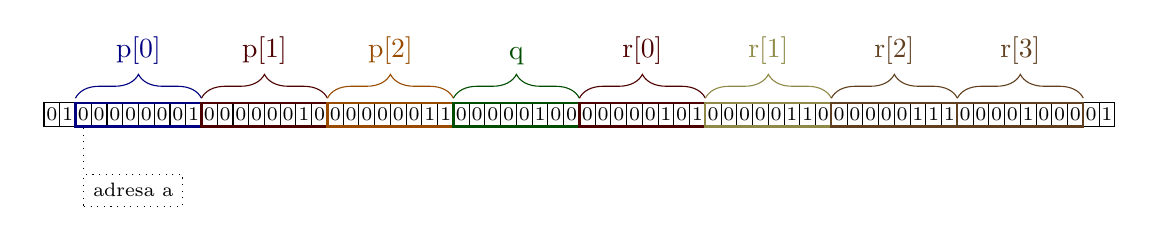
\begin{tikzpicture}[scale=0.2]
  \foreach \v [count=\i] in {
    0,1,
    0,0,0,0,0,0,0,1,
    0,0,0,0,0,0,1,0,
    0,0,0,0,0,0,1,1,
    0,0,0,0,0,1,0,0,
    0,0,0,0,0,1,0,1,
    0,0,0,0,0,1,1,0,
    0,0,0,0,0,1,1,1,
    0,0,0,0,1,0,0,0,
    0,1
  }{
    \draw (\i,0) rectangle node [anchor=center] {{\scriptsize\roboto \v}} (\i+1,1.5);
  }

  \var3{p[0]}{blue!50!black}
  \var{11}{p[1]}{red!30!black}
  \var{19}{p[2]}{orange!60!black}
  \var{27}{q}{green!30!black}
  \var{35}{r[0]}{red!30!black}
  \var{43}{r[1]}{yellow!50!black}
  \var{51}{r[2]}{brown!50!black}
  \var{59}{r[3]}{brown!50!black}
  
  \draw[dotted] (3.5,-0.1) -- (3.5,-3) 
  node[draw, anchor = north west]{\scriptsize adresa~\vb{a}};
\end{tikzpicture}}

Podobne keby som mal

\begin{lstlisting}
struct X {
  uint16_t x;
  uint8_t y, z[3];
  uint16_t w;
};

int main() { X x; }
\end{lstlisting}

tak v pamäti môžem mať \\

\centerline{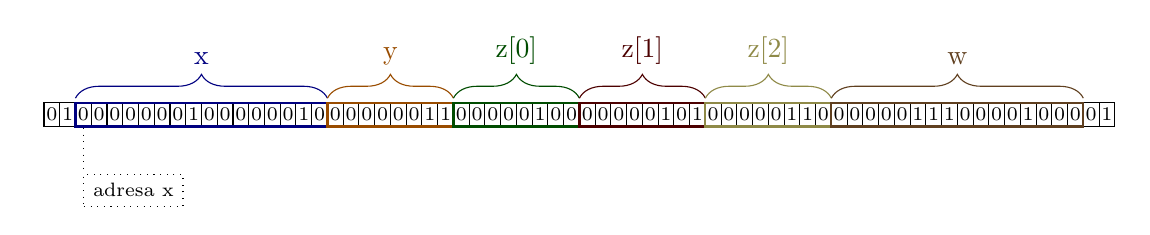
\begin{tikzpicture}[scale=0.2]
  \foreach \v [count=\i] in {
    0,1,
    0,0,0,0,0,0,0,1,
    0,0,0,0,0,0,1,0,
    0,0,0,0,0,0,1,1,
    0,0,0,0,0,1,0,0,
    0,0,0,0,0,1,0,1,
    0,0,0,0,0,1,1,0,
    0,0,0,0,0,1,1,1,
    0,0,0,0,1,0,0,0,
    0,1
  }{
    \draw (\i,0) rectangle node [anchor=center] {{\scriptsize\roboto \v}} (\i+1,1.5);
  }

  \varf3{x}{blue!50!black}
  \var{19}{y}{orange!60!black}
  \var{27}{z[0]}{green!30!black}
  \var{35}{z[1]}{red!30!black}
  \var{43}{z[2]}{yellow!50!black}
  \varf{51}{w}{brown!50!black}
  
  \draw[dotted] (3.5,-0.1) -- (3.5,-3) 
  node[draw, anchor = north west]{\scriptsize adresa~\vb{x}};
\end{tikzpicture}}

Ak si iteraz spravím

\begin{lstlisting}
union Z {
  A a;
  X x;
};

int main() { Z z; }
\end{lstlisting}

bude v pamäti\\

\centerline{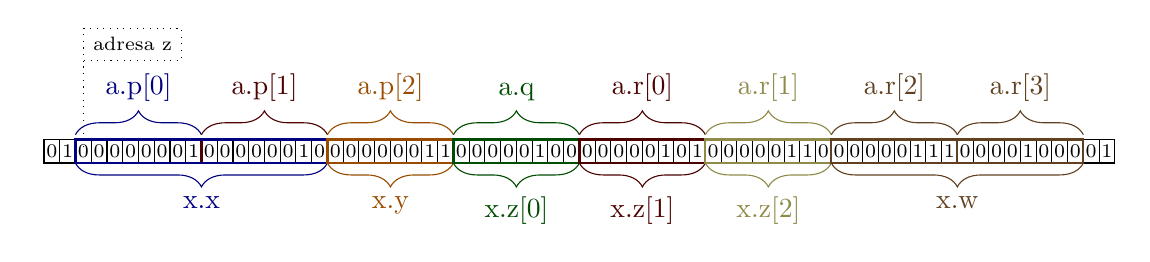
\begin{tikzpicture}[scale=0.2]
  \def\dvar#1#2#3{%
    \draw[#3] decorate[
       decoration={brace, amplitude=2ex, mirror}]{
       (#1,0) -- (#1+8,0) node [align=center,midway,anchor=north,yshift=-2ex] {\vb{#2}}
        };
   \draw[#3,thick] (#1,0) rectangle (#1+8,1.5);
  }

  \def\dvarf#1#2#3{%
    \draw[#3] decorate[
       decoration={brace, amplitude=2ex, mirror}]{
       (#1,0) -- (#1+16,0) node [align=center,midway,anchor=north,yshift=-2ex] {\vb{#2}}
        };
   \draw[#3,thick] (#1,0) rectangle (#1+16,1.5);
  }

  \foreach \v [count=\i] in {
    0,1,
    0,0,0,0,0,0,0,1,
    0,0,0,0,0,0,1,0,
    0,0,0,0,0,0,1,1,
    0,0,0,0,0,1,0,0,
    0,0,0,0,0,1,0,1,
    0,0,0,0,0,1,1,0,
    0,0,0,0,0,1,1,1,
    0,0,0,0,1,0,0,0,
    0,1
  }{
    \draw (\i,0) rectangle node [anchor=center] {{\scriptsize\roboto \v}} (\i+1,1.5);
  }

  \var3{a.p[0]}{blue!50!black}
  \var{11}{a.p[1]}{red!30!black}
  \var{19}{a.p[2]}{orange!60!black}
  \var{27}{a.q}{green!30!black}
  \var{35}{a.r[0]}{red!30!black}
  \var{43}{a.r[1]}{yellow!50!black}
  \var{51}{a.r[2]}{brown!50!black}
  \var{59}{a.r[3]}{brown!50!black}
  
  \dvarf3{x.x}{blue!50!black}
  \dvar{19}{x.y}{orange!60!black}
  \dvar{27}{x.z[0]}{green!30!black}
  \dvar{35}{x.z[1]}{red!30!black}
  \dvar{43}{x.z[2]}{yellow!50!black}
  \dvarf{51}{x.w}{brown!50!black}
  
  \draw[dotted] (3.5,1) -- (3.5,6.5) 
  node[draw, anchor = south west]{\scriptsize adresa \vb{z}};
\end{tikzpicture}}

Typ \vb{Z} má dve premenné: \vb{a}, ktorá je typu \vb{A} a \vb{x}, ktorá je typu \vb{X}. Obidve sú ale uložené v tom istom mieste v pamäti, takže ak 
napíšeš
\vb{z.a.q=10;}, tak vzápätí bude platiť \footnote{%
  Toto je definícia z jazyka C, kde sú veci zjednodušené tým, že tam neexistujú  metódy, konštruktory a pod. V C++ veci začnú byť zložitejšie: typy \vb{A} aj \vb{X}
  by mohli mať konštruktory a rôzne metódy, takisto \vb{Z} môže mať konštruktor a svoje metódy a potom je otázne, čo presne sa má stať, ak za napr. v premennej
  typu \vb{Z} zavolá
  konštruktor \vb{A} ale volá sa metóda \vb{X}. V C++ je preto zakázané čítať z typu \vb{union} inú premennú, ako tú, cez ktorú sa doňho zapisovalo. Celkovo použitie
  typu \vb{union} v C++ ti okrem veľmi špeciálnych prípadov neodporúčam, ako vraví známy citát: ``{\em Všetko môžem, ale nie všetko osoží}''. Ak potrebuješ schovať
  viac typov do jedného (napr. keď si navrhuješ nejaký protokol na komunikáciu), je lepšie použiť\indexItem{Prg}{typ \vb{std::variant}} 
  \vb{std::variant} zo štandardnej knižnice. My tu budeme
  používať typ \vb{union} iba pri \vb{SDL\_Event} v jeho základnej verzii bez konštruktorov a metód. 
} \vb{z.x.z[0]==10}.

 
Typ \vb{SDL\_Event} je definovaný asi takto:

\begin{lstlisting}
union SDL_Event {
    uint32_t type;                  // typ: podľa toho viem, kam sa mám pozerať
    SDL_MouseMotionEvent motion;    // pohyb myši
    SDL_MouseButtonEvent button;    // kliknutie
    SDL_KeyboardEvent key;          // stlačenie klávesy
    SDL_QuitEvent quit;             // zavretie okna zo systému
    SDL_WindowEvent window;         // zmeny veľkosti, umiestnenia, ... okna
    ....                            // atď, veľa ďalších typov
};
\end{lstlisting}

Všetky typy majú v pamäti na začiatku \vb{uint32\_t type}, takže ak mám premennú \vb{SDL\_Event e;} tak bez ohľadu na to, čo je v nej uložené, 
\vb{e.type} bude identifikátor typu\footnote{na to sú definované konštanty ako \vb{SDL\_QUIT}, \vb{SDL\_MOUSEMOTION}, \vb{SDL\_KEYDOWN} a pod., takže typický test je napr.
\prg!if (e.type == SDL_QUIT) running=false;!}. Jednotlivé typy majú tieto premenné:

\begin{lstlisting}
struct SDL_MouseMotionEvent {
    uint32_t type;       // SDL\_MOUSEMOTION 
    uint32_t timestamp   // čas, kedy udalosť vznikla
    uint32_t windowID;   // okno, ktoré má fokus
    uint32_t which;      // číslo myši alebo  SDL\_TOUCH\_MOUSEID  
    uint8_t state;       // stav gombíkov
    int32_t x;           // x-ová súradnica vzhľadom na okno
    int32_t y;           // y-ová súradnica vzhľadom na okno
    int32_t xrel;        // pohyb v smere osi x
    int32_t yrel;        // pohyb v smere osi y
};
\end{lstlisting}

\begin{lstlisting}
struct SDL_MouseButtonEvent {
    uint32_t type;       // SDL\_MOUSEBUTTONDOWN alebo SDL\_MOUSEBUTTONUP 
    uint32_t timestamp;  // čas, kedy udalosť vznikla
    uint32_t windowID;   // okno, ktoré má fokus
    uint32_t which;      // číslo myši alebo  SDL\_TOUCH\_MOUSEID
    uint8_t button;      // stav gombíkov
    uint8_t state;       // SDL\_PRESSED alebo SDL\_RELEASED 
    int32_t x;           // x-ová súradnica vzhľadom na okno
    int32_t y;           // y-ová súradnica vzhľadom na okno
};
\end{lstlisting}

\begin{lstlisting}
struct SDL_KeyboardEvent {
    uint32_t type;        // SDL\_KEYDOWN alebo SDL\_KEYUP 
    uint32_t timestamp;   // čas, kedy udalosť vznikla
    uint32_t windowID;    // okno, v ktorom je aktívny vstup
    uint8_t state;        // SDL\_PRESSED alebo SDL\_RELEASED
    uint8_t repeat;       // nenulové, ak vzniklo automatickým opakovaním
    SDL_Keysym keysym;    // klávesa
};
\end{lstlisting}

Stav gombíkov je bitové \vb{OR} z konštánt 
\vb{SDL\_BUTTON\_LMASK},
\vb{SDL\_BUTTON\_MMASK} a
\vb{SDL\_BUTTON\_RMASK}. Typ \vb{SDL\_KeyboardEvent} má premennú typu  \vb{SDL\_Keysym}. Ten je trochu zložitejší,\indexItem{Prg}{vstup z klávesnice} 
lebo dáva informáciu o fyzickej klávese
({\robotomono scancode},t.j. čudlík klávesnici) aj o logickej ({\robotomono keycode} t.j. znak).

\begin{lstlisting}
struct SDL_Keysym {
    SDL_Scancode scancode;      // kód fyzickej klávesy
    SDL_Keycode sym;            // kód logickej klávesy
    uint16_t mod;               // stlačené modifikátory
};
\end{lstlisting}

My budeme klávesnicu používať iba na zistenie, kedy sa stlačí nejaká klávesová kombinácia, čo sa dá napr. takto:

\begin{lstlisting}
if (e.type == SDL_KEYDOWN) {
  SDL_Keysym k = e.key.keysym;
  if (k.sym == SDLK_q && ((k.mod & (KMOD_LCTRL | KMOD_RCTRL)) != 0))
    running = false;
}
\end{lstlisting}

V tomto zápise \vb{KMOD\_LCTRL | KMOD\_RCTRL} je číslo, ktoré má nastavené bity (pomocou \vb{OR}) 
pre stlačenú ľavú a pravú klávesu {\robotomono Ctrl} a \vb{k.mod} má nastavené bity
stlačených modifikátorov. Preto \vb{(k.mod \& (KMOD\_LCTRL | KMOD\_RCTRL))} je číslo, ktoré má nastavené bity zodpovedajúce stlačeným {\robotomono Ctrl}; ak je nenulové,
nejaký {\robotomono Ctrl} je stlačený. Predchádzajúci kus programu preto testuje, či je stlačené {\robotomono Ctrl+Q}.

Len pre úplnosť dodám, že ak by si chcel načítavať text, ktorý používateľ píše, je lepšie namiesto \hbox{\vb{SDL\_KEYDOWN}} použiť udalosť \vb{SDL\_TEXTINPUT}
s príslušným typom \vb{SDL\_TextInputEvent e.text}. Ak chceš, naopak, zisťovať, ktoré klávesy sú práve stlačené (napr. chceš niečo ovládať šípkami),
je lepšie nečakať na udalosti a zavolať funkciu \link{https://wiki.libsdl.org/SDL2/SDL_GetKeyboardState}{SDL\_GetKeyboardState}.
V online dokumentácii SDL sú aj zoznamy konštánt pre \link{https://wiki.libsdl.org/SDL2/SDL_Keycode}{SDL\_Keycode} a \link{https://wiki.libsdl.org/SDL2/SDL_Keymod}{SDL\_Keymod}.

\vb{SDL\_WindowEvent} tu príliš rozoberať nebudeme, použijeme ho iba na to, aby sme vedeli zareagovať, keď sa zmení veľkosť okna. Aby sme to celé dali dokopy, ostáva predstaviť
funkciu na detekciu udalosti \hbox{\vb{SDL\_WaitEvent(SDL\_Event * event)},} 
ktorá zastaví program a čaká, 
kým nenastane nejaká udalosť, a potom ju uloží do premennej (ako parameter dostane pointer na 
ňu). Takže jednoduchý program \link{\rootpath/sdl/02/main.cc}{main.cc}, ktorý čaká na stlačenie {\robotomono Ctrl+Q} a pri každej udalosti prekreslí okno, by mohol vyzerať
takto:

\begin{lstlisting}
#include <SDL2/SDL.h>
#include <iostream>
using namespace std;

SDL_Window* window = nullptr;
SDL_Renderer* renderer = nullptr;

int main() {
  int ww = 800, wh = 600;
  SDL_Init(SDL_INIT_VIDEO | SDL_INIT_TIMER | SDL_INIT_AUDIO);
  window = SDL_CreateWindow("prvy pokus", SDL_WINDOWPOS_CENTERED,
                            SDL_WINDOWPOS_CENTERED, ww, wh,
                            SDL_WINDOW_RESIZABLE | SDL_WINDOW_SHOWN);
  renderer = SDL_CreateRenderer(window, -1, SDL_RENDERER_ACCELERATED);
  SDL_SetRenderDrawBlendMode(renderer, SDL_BLENDMODE_BLEND);

  bool running = true;
  SDL_Rect r{.x = 100, .y = 100, .w = 100, .h = 100};

  while (running) {
    SDL_Event e;
    SDL_WaitEvent(&e);  // počkaj na udalosť a ulož ju do premennej e

    if (e.type == SDL_WINDOWEVENT && e.window.event == SDL_WINDOWEVENT_SIZE_CHANGED) {
      ww = e.window.data1; // toto sú premenné z typu SDL\_WindowEvent,
      wh = e.window.data2; // v ktorých je nová veľkosť okna 
      cout << "nova velkost okna: " << ww << " x " << wh << endl;
    } else if (e.type == SDL_QUIT)
      running = false;
    else if (e.type == SDL_KEYDOWN) {
      SDL_Keysym k = e.key.keysym;
      cout << "stlacene: " << SDL_GetKeyName(k.sym) << ", mod " << k.mod << endl;
      if (k.sym == SDLK_q && ((k.mod & (KMOD_LCTRL | KMOD_RCTRL)) != 0))
        running = false;
    }
    // prekresli okno ako minule
    SDL_SetRenderDrawColor(renderer, 250, 180, 0, 255);
    SDL_RenderClear(renderer);
    SDL_SetRenderDrawColor(renderer, 20, 30, 180, 255);
    SDL_RenderFillRect(renderer, &r);
    SDL_RenderPresent(renderer);
  } // koniec while-cyklu, zatvoríme okno a končíme

  SDL_DestroyWindow(window);
  SDL_Quit();
}
\end{lstlisting}

Tu si môžeš všimnúť typickú štruktúru grafických programov: v premenných máme uložené,
čo sa má kam zobraziť. V cykle vždy spracujeme udalosť, aktualizujeme premenné
a nakoniec prekreslíme obrazovku.

\begin{uloha}
  \label{uloha:SDL.stvorec1}
  Napíš program, v ktorom bude používateľ môcť modrý štvorec premiestňovať myšou:
  keď klikne myšou na štvorec, prejde sa do režimu ťahania, v ktorom štvorec 
  sleduje kurzor, až kým používateľ nepustí gombík myši. Zároveň treba zabezpečiť, aby
  štvorec nikdy netrčal mimo okna a pri zmene veľkosti okna sa vždy posunul tak, aby bol celý 
  viditeľný.
\end{uloha}

\indexItem{Prg}{príkaz \vb{switch}}
Tu urobím ešte jednu odbočku a ukážem ti príkaz \vb{switch}. Doteraz som ti ho neukázal,
lebo nie je na písanie programov nevyhnutný, ale ak si budeš niekedy pozerať programy, hlavne 
také, ktoré používajú knižnice ako SDL, určite sa s ním stretneš. Všimni si, že v 
predchádzajúcom programe je pomerne typická konštrukcia

\begin{lstlisting}
if (x == 0) kvak(); 
else if (x == 1) kvik();
else if (x == 2) kvok();
else if (x == 3) kvuk();
...
\end{lstlisting}

keď veľakrát za sebou testujem tú istú premennú na rôzne hodnoty. 
Príkaz \vb{switch(x)} bude nasledovaný zloženým príkazom, ktorý obsahuje tzv. 
{\em návestia} \vb{case} pre rôzne hodnoty. Zoberme si funkciu

  \begin{lstlisting}
void f(int x) {
  switch (x) {
    case 0:
      cout << "0 ";
    case 1:
      cout << "1 ";
    case 2:
      cout << "2 ";
    case 3:
      cout << "3 ";
    case 4:
      cout << "4 ";
    case 5:
      cout << "5 ";
      break;
    case 6:
      cout << "6 ";
    case 7:
      cout << "7 ";
    case 8:
      cout << "8 ";
    case 9:
      cout << "9 ";
  } 
}
  \end{lstlisting}

  Keď zavolám \prg!f(x)!, v príkaze \vb{switch(x)} sa vyhodnotí výraz \vb{x}
  a začne sa vykonávať zložený príkaz od toho \vb{case}, ktoré má rovnakú hodnotu
  až do konca. Príkaz \vb{break} v tomto prípade preruší vykonávanie. Preto napr.
  \vb{f(3)} začne vykonávať príkazy od \vb{case 3:} a skončí tesne pred \vb{case 6:},
  lebo tam nazarí na \vb{break}. Program

\begin{lstlisting}
int main() {
  for (int i=0; i<10; i++) { 
    f(i); 
    cout << endl; 
  }
}
\end{lstlisting}

by napísal

\begin{outputBox}
0 1 2 3 4 5 
1 2 3 4 5 
2 3 4 5 
3 4 5 
4 5 
5 
6 7 8 9 
7 8 9 
8 9 
9
\end{outputBox}

Koniec odbočky, vráťme sa ku grafike s SDL. Máme základnú schému programu, ktorá vyzerá zhruba takto:

\vbox{
\begin{lstlisting}
int main() {
  SDL_Init(...);
  ...                   // nastaviť všetko, čo na začiatku treba

  bool running = true;  
  while (running) {     // kým netreba skončiť

    SDL_Event e;
    SDL_WaitEvent(&e);  // počkaj na udalosť

    switch (e.type) {   // spracuj rôzne typy udalostí
      case SDL_QUIT:
        running = false;
        break;
      case SDL_MOUSEMOTION:
        ...            
        break;
      ...
    }

    SDL_SetRenderDrawColor(renderer, 250, 180, 0, 255); // zmaž pozadie
    SDL_RenderClear(renderer);
    ...                                                 // nakresli všetko, čo treba
    SDL_RenderPresent(renderer);
  }
}
\end{lstlisting}
}

Teraz chcem upraviť program z 
Úlohy~\ref{uloha:SDL.stvorec1} tak, aby modrý štvorec pulzoval: 
plynule menil farbu aj veľkosť. Aby som si udržal poriadok v programe, budem si držať všetko, čo potrebujem na vykreslenie štvorca, v jednej premennej,
ktorá bude mať metódu \vb{render(SDL\_Renderer *)} (t.j. ako parameter dostane pointer na renderer, a ním sa vykreslí). Na zmenu farby použijem triedu
\vb{Gradient} z Úlohy~\ref{uloha:gradient}. Pretože budem chcieť meniť veľkosť štvorca, budem si pamätať jeho pozíciu \vb{cx}, \vb{cy}  a rozmery 
(\vb{w}$\times$\vb{h}). Ešte si môžem vyrobiť pomocnú funkciu \vb{contains}, ktorá mi povie, či bod so súradnicami $x,y$ leží vnútri štvorca.\\

\begin{lstlisting}
struct Stvorec {
  int cx = 100, cy = 100, w = 100, h = 100;
  Gradient gradient;
  Stvorec(const Gradient& _g) : gradient{_g} {}  // konštruktor dostane gradient
  void render(SDL_Renderer* renderer);           // zobrazovacia funkcia
  bool contains(int x, int y) { 
    return (abs(x - cx) < w / 2 && abs(y - cy) < h / 2); 
  }
};
\end{lstlisting}

\indexItem{Prg}{\vb{SDL\_GetTicks}, \vb{SDL\_Delay}, \vb{SDL\_PollEvent}}
Na vykreslenie štvorca budem potrebovať hodinky, aby mohol pravidelne pulzovať. Môžem použiť tie z kapitoly~\ref{sect:clock}, ale SDL má aj 
vlastnú implementáciu \vb{uint32\_t SDL\_GetTicks()}, ktorá vráti počet milisekúnd od spustenia programu. 
Keď potrebujem niečo pravidelne opakovať každých \vb{s} milisekúnd a napíšem \prg!SDL_GetTicks() % s!, tak dostanem číslo, ktoré sa pravidelne mení v rozsahu
$0$ až \vb{s} každú milisekundu. Keď potom napíšem \prg!(double)(SDL_GetTicks() % s) / (double)s!,
budem mať číslo, ktoré sa pravidelne mení medzi $0$ a $1$ za \vb{s} milisekúnd. 
Renderovacia funkcia by mohla vyzerať takto:

\vbox{
\begin{lstlisting}[label={l:sdl.2}]
void Stvorec::render(SDL_Renderer* renderer) {
  uint32_t now = SDL_GetTicks();    // zisti čas

  // nastav farbu podľa gradientu (potrebujem ho mať symetrický)
  Vec3 clr = gradient((double)(now % 10000) / 10000.0L);  // jeden cyklus bude 10s
  // renderer chce uint8\_t, ja mám reálne čísla medzi 0..1, takže prenásobím
  SDL_SetRenderDrawColor(renderer, 255 * clr.x, 255 * clr.y, 255 * clr.z, 255);

  SDL_Rect r; // obdĺžnik, ktorý budeme renderovať
  double a = 0.8 * (1.0 + sin(2.0 * M_PI * (double)(now % 340) / 340.0L)); @\ll1@
  r.x = cx - w / 2 + a;
  r.y = cy - h / 2 + a;
  r.w = w - 2 * a;
  r.h = h - 2 * a;

  SDL_RenderFillRect(renderer, &r);
}
\end{lstlisting}
}


\begin{column}{0.5}
Na riadku~\ref{l:sdl.2-1} rátam hodnotu \vb{a}, o ktorú sa zmenšia rozmery štvorca. Aby sa menili plynule, použil som funkciu \vb{sin} (treba \prg!#include <cmath>!),
ktorá robí ``vlnku'' na intervale $[0,2\pi]$. Keď mám $x$ z intervalu $[0,1]$, tak na vlnku potrebujem funkciu $\sin(2\pi x)$. Tá má ale hodnoty od $-1$ po $1$,
takže $1+\sin(2\pi x)$ bude mať hodnoty od $0$ po $2$ a bude vyzerať takto:
\end{column}\hspace*{1cm}\begin{column}{0.5}
\begin{tikzpicture}
\begin{axis}[
 height=5cm,   
 trig format plots=rad,
  width=\textwidth
]
\addplot [
red,
domain=0:1,
samples=201,
]
  {1+sin(2*3.1415926535*x)};
\end{axis}
\end{tikzpicture}
\end{column}

Hlavný cyklus ale teraz musím urobiť inak. Keďže \vb{SDL\_WaitEvent} čaká na udalosť, štvorec by sa menil iba kým by si hýbal myšou (alebo iným spôsobom vyrábal udalosti).
Existuje ale podobná funkcia \vb{SDL\_PollEvent}, ktorá na nič nečaká, ale ak je nejaká udalosť pripravená v poli udalostí, skopíruje ju do zadaného pointra a vráti \vb{true}, inak vráti
\vb{false}. Keďže udalostí môže nastať aj viacero naraz, typický hlavný cyklus vyzerá takto:\\

\begin{lstlisting}
  while (running) {
    SDL_Event e;

    while (SDL_PollEvent(&e)) { // spracuj všetky udalosti, kým sú
      switch (e.type) {
        case SDL_QUIT:
          running = false;
          break;
        case SDL_MOUSEMOTION:
          ...
          break;
        ...
      }
    }

    // prekresli okno
  }
\end{lstlisting}

Posledná vec, ktorú treba spomenúť je efektivita. Takto napísaný cyklus beží stále dokola na plný výkon počítača. To nie je ideálne, hlavne na notebooku to veľmi rýchlo minie
baterku. Preto je slušné obmedziť počet snímkov za sekundu ({\em frames per second}, \prg!fps!). Na začiatku vykresľovania si odmeriam čas pomocou 
\hbox{\vb{SDL\_GetTicks}.} Rovnako urobím aj na konci a zistím, koľko milisekúnd trvalo vykresľovanie. Ak chcem mať fixné \prg!fps!, vykresliť jeden snímok má 
trvať \prg!1000/fps! milisekúnd. Ak som bol s vykresľovaním hotový skôr, počkám potrebný počet milisekúnd pomocou \vb{SDL\_Delay}. Skús si to, čo sme
tu teraz hovorili, naprogramovať:

\begin{uloha}
  Uprav Úlohu~\ref{uloha:SDL.stvorec1} tak, aby štovrec pulzoval a menil farby.
\end{uloha}

\section*{Práca s obrázkami}

\indexItem{Prg}{\vb{SDL\_Surface} a \vb{SDL\_Texture}, \vb{SDL\_Image}}
Pomocou SDL sa dajú priamo vykresľovať útvary zložené z čiar, bodov a obdĺžnikov, ale 
hlavná sila SDL je v práci s obrázkami. V knižnici sú dva hlavné typy, ktoré vedia s
obrázkami pracovať \hbox{\vb{SDL\_Surface}} a \hbox{\vb{SDL\_Texture}.}

\vb{SDL\_Surface} je vlastne pole pixelov v pamäti. Je to trošku komplikovanejšie, lebo
pixely môžu byť uložené rôzne (napr. RGB, RGBA, ako odtiene sivej, ako indexy do palety, ...).
Premenná \vb{format} popisuje, akým spôsobom treba k pixelom pristupovať.

\begin{lstlisting}
struct SDL_Surface {
    SDL_PixelFormat *format;    // spôsob uloženia pixelov
    int w, h;                   // rozmery
    int pitch;                  // dĺžka riadka v bytoch
    void *pixels;               // pole pixelov
    void *userdata;             // sem si môžeš zapísať, čo chceš
    SDL_Rect clip_rect;         // mimo tohoto obdĺžnika sa nekreslí
    ...                         // atď.
};
\end{lstlisting}

Naproti tomu \vb{SDL\_Texture} je tiež pole pixelov, ale kde je uložené, to závisí od 
konkrétneho systému. Ak to totiž hardvér podporuje, pole sa umiestni do pamäti  grafickej karty. To znamená,
že z programu nemôžeš priamo pristupovať k jednotlivým pixelom, ale prekresľovanie je 
oveľa rýchlejšie, lebo si to grafická karta vie zariadiť sama. Dáta z pamäte vieš poslať
na kartu
pomocou \vb{SDL\_CreateTextureFromSurface}), ale naopak to nejde.

SDL samotná podporuje iba obrázkový formát \vb{.bmp}. Ak chceš pracovať aj s inými,
treba použiť rozšírenie \vb{SDL\_Image}. To znamená v programe pridať 
\prg!#include <SDL2/SDL_image.h>!, v \vb{Makefile} pridať pri linkovaní \vb{-lSDL2\_image}
a možno rozšírenie aj nainštalovať (napr. \vb{sudo apt-get install libsdl2-image-dev}).

Pri písaní programu treba po zavolaní \vb{SDL\_Init} zvoliť, aké formáty sa majú používať, napr.
\vb{IMG\_Init(IMG\_INIT\_PNG);} a na konci programu, pred volaním \vb{SDL\_Quit()}
treba zavolať \vb{IMG\_Quit()}. Ak chceš, aby správne fungovali transparentné pixely
({\em alpha channel}), treba predtým zapnúť
\hbox{\vb{SDL\_SetRenderDrawBlendMode(renderer, SDL\_BLENDMODE\_BLEND);}}


Na prečítanie obrázku zo súboru sú dve funkcie, ktoré robia presne to, čo hovorí definícia (t.j. zoberie súbor s daným menom a vyrobí textúru alebo surface):

\begin{lstlisting}
SDL_Surface * IMG_Load(const char *file);
SDL_Texture * IMG_LoadTexture(SDL_Renderer *renderer, const char *file);
\end{lstlisting}

Keď už máš textúru v pamäti karty (t.j. v premennej typu \vb{SDL\_Texture}), dá sa vykresliť pomocou funkcií

\begin{lstlisting}
SDL_RenderCopy( SDL_Renderer *, SDL_Texture *, SDL_Rect *src, SDL_Rect *dst );

SDL_RenderCopyEx( SDL_Renderer *, SDL_Texture *, SDL_Rect *src, SDL_Rect *dst,
                  double angle, SDL_Point *center, int flip);                
\end{lstlisting}

Čo presne robia? Prvé dva parametre sú jasné: renderer, ktorý má vykresľovať a textúra, ktorú treba vykresliť. Druhé dva parametre sú pointre na obdĺžniky. Z textúry 
sa zoberie obdľžnik \vb{src} a vyrenderuje sa na pozíciu \vb{dst} (ak treba, tak sa naškáluje\footnote{Na presnejšie, ale pomalšie škálovianie 
sa dá zavolať \prg!SDL_SetHint(SDL_HINT_RENDER_SCALE_QUALITY, "2");!.})

Napríklad ak mám textúru s obrázkom  \link{\rootpath/sdl/03/penguin.png}{tučniaka}, načítam si ju pomocou

\begin{lstlisting}
SDL_Texture* penguin = IMG_LoadTexture(renderer, "penguin.png");
\end{lstlisting}

Ak z nej potom vyberiem obdĺžnik \vb{src} a vyrenderujem ho 
pomocou \vb{SDL\_RenderCopy} do okna na obdĺžnik \vb{dst}, dotsanem niečo takéto:\\

\centerline{
\begin{tikzpicture}[scale=0.6]
  \definecolor{darkyellow}{RGB}{250,180,0}
  \def\peng{\draw[fill stretch image=data/penguin.png] (0,0) rectangle (7.62,10.02);}
  \def\rect{(0.5,0.11) rectangle (7,3)}
  \peng
  \draw[thick,red] \rect;
  \node  [above=1ex, anchor=south, red] at (3.75,3)  {{\robotomono src}};
  \node [above=1ex, anchor=south] at (0.5*7.62,10.02) {{\robotomono texture}};

  \begin{scope}[shift={(11,0)}]
    \fill[draw=black, fill=darkyellow] (0,0) rectangle (12,9);
    \node  [above=1ex, anchor=south] at (6,9) {{\robotomono window}};
    \begin{scope}[shift={(5,1.8)}, xscale=0.5, yscale=1.75]
    \draw[thick,red]\rect;
      \node [above=1ex, anchor=south, red] at (3.75,3) {{\robotomono dst}};  
    \clip \rect;  
    \draw[thick,red]\rect;
    \peng
    \end{scope}
  \end{scope}
\end{tikzpicture}
}

Keby som chcel vykresliť celého tučniaka do stredu okna (celý program je  \link{\rootpath/sdl/03/main.cpp}{tu}), budem mať

\begin{lstlisting}
    SDL_SetRenderDrawColor(renderer, 250, 180, 0, 255);
    SDL_RenderClear(renderer);
    //  umiestnenie tučniaka v textúre
    SDL_Rect src{.x = 0, .y = 0, .w = 722, .h = 1002};  
    
    // ww a wh sú rozmery okna, chcem sa naškálovať na 90\% menšieho z nich
    double scale = 0.9 * min((double)ww / 722.0, (double)wh / 1002.0);

    int nw = scale * 722, nh = scale * 1002;            //  rozmery tučniaka v okne 
    SDL_Rect dst{.x = (ww - nw) / 2, .y = (wh - nh) / 2, .w = nw, .h = nh};
    SDL_RenderCopy(renderer, penguin, &src, &dst);
    SDL_RenderPresent(renderer);
\end{lstlisting}

Druhá funkcia, \vb{SDL\_RenderCopyEx} je podobná, iba navyše môže obrázok aj zrotovať okolo bodu \vb{center} o \vb{angle} stupňov v smere hodinových ručičiek
a zrkadlovo prevrátiť.
Parameter \vb{flip} je bitové \vb{OR} z konštánt \vb{SDL\_FLIP\_NONE}, \vb{SDL\_FLIP\_HORIZONTAL} a \vb{SDL\_FLIP\_VERTICAL}.
Ak namiesto niektorého obdĺžnika zadám \vb{nullptr}, berie sa celá textúra, resp. celé okno.

Ak už surface, resp. textúru nepotrebuješ, treba ručne zavolať ``deštruktor'' \vb{SDL\_FreeSurface(surf)} resp. \vb{SDL\_DestroyTexture(txt)}.

\begin{uloha}
  Textúra tučniaka má od pozície $(722,0)$ snehovú vločku rozmerov $40\times40$. Napíš program, ktorý vykreslí tučniaka v strede okna a za ním bude snežiť (t.j. bude
  tam veľa snehových vločiek padať zhora dolu).
\end{uloha}

\begin{uloha}
  Na stránke 
  \link{https://sanderfrenken.github.io/Universal-LPC-Spritesheet-Character-Generator}{Spritesheet Character Generator} si vytvor postavu a stiahni si \vb{.png} obrázok s rozfázovaným
  pohybom, tzv. {\em spritesheet}. Urob program, v ktorom postava chodí po obrazovke a  ovládaš\footnote{%
    Ako som spomínal, je lepšie nespoliehať sa na udalosti, ale priamo kontrolovať,
    ktoré klávesy sú stlačené. Ak zavoláš \prg!const uint8_t *keys = SDL_GetKeyboardState(nullptr);!
    budeš mať pole, v ktorom je pre každý scancode jednotka, ak je daná klávesa stlačená a 0 ak nie je.
    Preto vieš zisťovať napr. \prg!if (keys[SDL_SCANCODE_DOWN] == 1) {...}!.
  }ju šípkami.
\end{uloha}

\section*{Písanie textu, fonty}
\indexItem{Prg}{fonty a text}

Na vykresľovanie textu potrebuješ font, t.j. (spravidla vektorový) popis, ako vyzerajú jednotlivé písmenká. Veľmi častý formát na ukladanie fontov je \vb{TrueType}, súbory majú príponu \vb{.ttf}. Je veľmi veľa miest, kde
sa dajú nájsť a stiahnuť voľne prístupné súbory \vb{.ttf}. Na vykresľovanie bude treba, aby si si svoj obľúbený font našiel a dal do pracovného adresára. Ja budem používať font 
\link{https://github.com/JulietaUla/Montserrat/tree/master}{Montserrat}.

Na prácu s TrueType fontami je v SDL samostatné rozšírenie, ktoré treba, podobne ako prácu s obrázkami inicializovať: pridať \prg!#include <SDL2/SDL_ttf.h>!, v \vb{Makefile} pri linkovaní pridať \vb{-lSDL2\_ttf}
a možno ho predtým zvlášť nainštalovať, napr. \vb{sudo apt-get istall libsdl2-ttf-dev}. Rovnako, podobne ako pri rozšírení \vb{IMG}, treba na začiatku programu zavolať
\vb{TTF\_Init()} a na konci \vb{TTF\_Quit()}. Zoznam všetkých funkcií v rozšírení \vb{TTF} je \link{https://wiki.libsdl.org/SDL2_ttf/CategoryAPI}{tu}.

Prvá vec, ktorú treba s fontom urobiť, je nahrať ho do pamäte volaním

\begin{lstlisting}
TTF_Font *font =  TTF_OpenFont("Montserrat-Bold.ttf", 50);
\end{lstlisting}

Prvý parameter je meno súboru, druhý je veľkosť. Keď už font netreba, dá sa odstrániť volaním ``deštruktora'' \vb{TTF\_CloseFont(font)}.
Keď mám font, môžem vyrenderovať text v nejakej farbe pomocou

\begin{lstlisting}
SDL_Surface * TTF_RenderUTF8_Blended(TTF_Font *font, const char *text, SDL_Color fg);
\end{lstlisting}

Podobných funkcií je niekoľko, líšia sa tým, ako je zadaný text (v našom prípade mám \vb{UTF-8}, čo je bežné kódovanie pre texty s diakritikou) a ako kvalitne (tým pádom aj pomaly)
sa má renderovať (v našom prípade má brať do úvahy transparentnosť). Dostaneme bitmapový obrázok v pamäti (\vb{SDL\_Surface} má, okrem iného, premenné \vb{w} a \vb{h}, 
ktoré udávajú rozmery. Bez toho, aby sme text naozaj renderovali, vieme zistiť jeho rozmery volaním \vb{TTF\_SizeText(font, text, \&w, \&h)}).
Na vykreslenie potom musíme obrázok poslať na grafickú kartu, t.j. vyrobiť \vb{SDL\_Texture}, a vykresliť ho ako každú inú textúru. Ak chceme text renderovať veľakrát, 
vyrobený \vb{SDL\_Surface} a \vb{SDL\_Texture} si môžeme odložiť. Jednoduchá trieda na písanie textov by mohla vyzerať takto:\\

\begin{lstlisting}
struct Text {
  SDL_Surface *surf;
  SDL_Texture *txt;
  SDL_Rect box;

  Text(SDL_Renderer *renderer, TTF_Font *font, const char *text,
       SDL_Color color) {
    surf = TTF_RenderUTF8_Blended(font, text, color);
    box.h=surf->h;
    box.w=surf->w;
    txt = SDL_CreateTextureFromSurface(renderer, surf);
  }

  void render(SDL_Renderer *renderer, int x, int y) {
    box.x=x;
    box.y=y;
    SDL_RenderCopy(renderer, txt, nullptr, &box);
  }

  ~Text() {
    SDL_DestroyTexture(txt);
    SDL_FreeSurface(surf);
  }
};
\end{lstlisting}

Použili by sme ju napr.

\begin{lstlisting}
  TTF_Font *font = TTF_OpenFont("Montserrat-Bold.ttf", 50);
  Text t(renderer,font,"môj täxt",SDL_Color{.r=10,.g=80,.b=150});
  ...
  while (running) {
    ...
    t.render(renderer,x,y);
    ...
  }
\end{lstlisting}

\begin{uloha}
  Napíš program, ktorý prečíta zo vstupu text a potom ho donekonečna v okne skroluje zľava doprava (keď zájde za pravý okraj, znovu vyjde spoza ľavého).
\end{uloha}

Nielen pri renderovaní textu sa hodí mať kontrolu nad cieľovým obdĺžnikom, do ktorého 
sa vykresľuje. Dá sa to síce urobiť pri volaní \vb{SDL\_RenderCopy}, ale ak
máš viacero vykresľovaní za sebou, je príjemné zavolať
\vb{SDL\_RenderSetClipRect(SDL\_Renderer *, SDL\_Rect *)}. Tým nastavíš orezávanie 
({\em clipping}) a všetky ďalšie príkazy budú vykresľovaiť iba do zadaného obdĺžnika. Keď
potom zavoláš \vb{SDL\_RenderSetClipRect}, kde druhý parameter bude \prg!nullptr!,
orezávanie sa vypne a vykresľovať sa bude opäť všetko.

\section*{Ako pridať zvuk}
\indexItem{Prg}{zvuk}

Aj keď sa to možno nezdá, prehrávanie zvuku môže byť pomerne komplikovaná záležitosť. SDL vie elegantne
zkryť všetky technické ťažkosti použitím ďalšieho (už posledného) rozšírenia: \vb{SDL\_Mixer}.
Nainštaluje sa rovnako, ako \vb{SDL\_Image} a \vb{SDL\_TTF}: do programu sa pridá
\prg!#include <SDL2/SDL_mixer.h>!, v \vb{Makefile} sa prilinkuje \vb{-lSDL2-mixer} (a, samozrejme,
nainštaluje sa príslušná knižnica, napr. \vb{libsdl2-mixer-dev}).

\vb{SDL\_Mixer} pridáva dva hlavné typy pre zvuk: \vb{Mix\_Chunk} a \vb{Mix\_Music}. Rozdiel 
medzi nimi je v tom, že \vb{Mix\_Chunk} sa celý dekóduje do pamäte, kým 
\vb{Mix\_Music} sa priebežne dekóduje pri prehrávaní z disku. 
\vb{Mix\_Chunk} na jednej strane zaberá miesto 
v pamäti, na druhej strane sú operácie ako zastavenie, skok na začiatok a pod. rýchlejšie.
\vb{Mix\_Chunk} sa preto používa na krátke zvukové efekty, kým napr. na hudbu na pozadí by si
radšej použil \vb{Mix\_Music}.

\vb{Mix\_Chunk}  sa prehráva v stopách ({\em channels}), pričom v jednej stope môže naraz hrať jeden zvuk. Môžeš si vyrobiť viacero stôp, aby mohlo hrať viacero efektov naraz,
ale \vb{Mix\_Music} vždy hrá najviac jedna.

Na začiatku treba inicializovať knižnicu napr. 
\begin{lstlisting}
Mix_OpenAudio(44100, MIX_DEFAULT_FORMAT, 2, 1024);
\end{lstlisting}
Pre vysvetlenie (ale asi to nebudeš potrebovať meniť):
prvvý parameter je vzorkovacia frekvencia, druhý je formát, tretí je počet kanálov (dva pre štandardné dvokjkanálové stereo) a posledný parameter je veľkosť
interného buffera pri prehrávaní. Po tom, ak inicializuješ audio, chceš vyrobiť stopy, v ktorých budeš prehrávať zvuky:
\begin{lstlisting}
Mix_AllocateChannels(nChannels);
\end{lstlisting}

Ďalšie použitie je pomerne priamočiare, tu je zopár funkcií, ktoré môžeš chcieť použiť (kompletný zoznam je \link{https://wiki.libsdl.org/SDL2_mixer/CategoryAPI}{tu}.

\def\mynl{\vspace{2ex}\linebreak}
\begin{tabularx}{\textwidth}{X}\toprule
  \vb{Mix\_Chunk * Mix\_LoadWAV(const char *file)}\\
  \vb{Mix\_Music * Mix\_LoadMUS(const char *file)}\\
  ``Konštruktor'': prečíta zvuk zo súboru\\\midrule
   \vb{int Mix\_PlayChannel(int channel, Mix\_Chunk *chunk, int loops)}\\
   \vb{int Mix\_PlayMusic(Mix\_Music *music, int loops)}\\
   Začne hrať zvuk. Pre \vb{chunk} parameter \vb{channel} udáva stopu, kde sa má zvuk hrať. Ak 
   je \vb{channel == -1} začne hrať na prvej voľnej stope. \vb{loops} je počet opakovaní: 0 znamená 
   \cmd{zahraj raz a skonči}, -1 znamená \cmd{stále opakuj}\\\midrule
%
  \vb{int Mix\_MasterVolume(int volume)}\\
  \vb{int Mix\_Volume(int channel, int volume)}\\
  \vb{int Mix\_VolumeMusic(int volume)}\\
  Nastaví hlasitosť v rozmedzí  \vb{0} a  \vb{MIX\_MAX\_VOLUME}.
  Ak je parameter \vb{volume} záporný, funkcia vráti súčasnú hlasitosť a nič nezmení.\\\midrule
%
  \vb{void Mix\_Pause(int channel)}\\
  \vb{void Mix\_PauseAudio(int pause\_on)}\\
  \vb{void Mix\_PauseMusic(void)}\\
  \vb{void Mix\_Resume(int channel)}\\
  \vb{void Mix\_ResumeMusic(void)}\\
  Preruší a pokračuje v prehrávaní.\\\midrule
%
  \vb{double Mix\_GetMusicPosition(Mix\_Music *music)}\\
  \vb{void Mix\_RewindMusic(void)}\\
  \vb{int Mix\_SetMusicPosition(double position)}\\
  Zistí pozíciu (v sekundách), pretočí na začiatok, prípadne skočí na danú pozíciu.\\\midrule
%
  \vb{int Mix\_HaltMusic(void)}\\
  \vb{int Mix\_HaltChannel(int channel)}\\
  Zastaví prehrávanie. Ak je \vb{channel == -1}, zastavia sa všetky stopy.\\\midrule
%
  \vb{void Mix\_HookMusicFinished(void (SDLCALL *music\_finished)(void))}\\
  \vb{void Mix\_ChannelFinished(void (SDLCALL *channel\_finished)(int channel))}\\
  Pointer na funkciu (ako v kapitole~\ref{sec:lambdy}), ktorá sa spustí, keď hudba dohrá. Môže napr. spustiť ďalšiu skladbu volaním \vb{Mix\_PlayMusic}\\\midrule
%
  \vb{void Mix\_FreeChunk(Mix\_Chunk *chunk)}\\
  \vb{void Mix\_FreeMusic(Mix\_Music *music)}\\
  ``Deštuktory''.
  \\\bottomrule
\end{tabularx}


\section*{Grafické prostredie pre \btr}

Teraz je už všetko pripravené na to, aby si napísal prvú verziu grafického prostredia pre \btr.
Chceme, aby to fungovalo takto: v zadanom obdĺžniku niekde v okne sa zobrazuje šachovnica (reaguje na zmenu veľkosti okna) s rozohratou pozíciou.
Hráč môže kedykoľvek chytiť myšou nejaký svoj kameň a pohybovať ním (možno sa zvýrazňuje políčko, odkiaľ kameň zobral a kde je práve teraz). Keď kameň
pustí, vráti sa na pôvodné miesto. Ak ale kameň pustí vtedy, keď je na ťahu a vyrobí sa prípustný ťah, tento ťah sa vykoná a aktualizuje sa pozícia.
Potom sa zistí ťah počítača a začne sa animovať plynulý presun kameňa (ťah sa tiež môže zvýrazniť), Keď kameň príde na svoje miesto, aktualizuje sa pozícia
a opäť je na ťahu hráč. Screenshot by mohol vyzerať asi takto:\\

\centerline{\includegraphics[width=0.4\textwidth]{data/guibtr.png}}

Naprogramujme to tak, že budeme mať triedu \vb{BoardView}, ktorá sa bude starať o vykresľovanie. Bude si pamätať obdĺžnik
\vb{SDL\_Rect screen}, do ktorého sa bude vykresľovať. Pre pohodlie si môže pamätať aj 
\vb{renderer}, keďže ju nikdy nebudeme chcieť renderovať inam. Premenná \vb{screen} sa bude meniť
volaním \vb{resize}. To je preto, že pri zmene veľkosti si možno budeš chcieť prepočítať
nejaké ďalšie veci, ktoré s veľkosťou okna súvisia. Napríklad rozmer šachovnice môžeš
nastaviť ako menší z dvoch rozmerov okna a pod. Bude si pamätať aj \link{\rootpath/sdl/pieces.png}{obrázok} hracích kameňov, 
aktuálnu polohu myši, či práve používateľ presúva kameň, či sa práve animuje a ak áno tak odkiaľ a kam atď. 
Hodia sa aj pomocné funkcie, ktoré pre políčko šachovnice vrátia pozíciu na obrazovke a naopak.
Jadro triedy by mohlo vyzerať takto:

\begin{lstlisting}
struct BoardView {
  SDL_Renderer* renderer;
  Board board;          // aktuálna pozícia
  SDL_Texture* pieces;  // textúra s bielym a čiernym kameňom
  uint8_t human;        // človek je Biely(0) / Čierny (1)
  bool flippedBoard;    // zobrazujem šachovnicu z pohľadu čierneho

  bool dragging, animating;  // ťahá hráč / počítač
  Square dragOrig;           // odkiaľ hráč začal ťah
  Move aMove;                // počítačový ťah, ktorý sa animuje
  const int animLen = 200;   // dĺžka animácie (ms)
  uint32_t animEndTime;      // kedy skončí aktuálna animácia

  SDL_Rect screen;     // obdĺžnik, kam sa vykresľujem
  int mouseX, mouseY;  // poloha myši
  ...                  // rôzne veci, ktoré potrebuješ pri vykresľovaní

  BoardView(SDL_Renderer* r);       // konštruktor
  void resize(SDL_Rect scr);        // nastaví všetko potrebné pri zmene okna
  void render();
  void operator+=(const Move& m);   // spustí animáciu ťahu protihráča

  void onMouseMotion(SDL_MouseMotionEvent& e);
  void onMouseDown(SDL_MouseButtonEvent& e);
  Move onMouseUp(SDL_MouseButtonEvent& e);
  ...                               // deštruktor, pomocné funkcie atď
};
\end{lstlisting}

V hlavnom cykle sa pri spracovaní eventov zavolajú funkcie \vb{onMouse...}, ktoré nastavia \vb{mouseX}, \vb{mouseY} a ošetria prípadný začiatok a koniec ťahania.
Špeciálne ak sa v \vb{onMouseUp} urobí ťah, tento sa vráti (inak vracia nejaký neprípustný ťah ako zarážku). V hlavnom programe sa tento ťah podhodí \vb{RandomPlayer}
z úlohy~\ref{uloha:randomplayer}, ktorý nájde ťah. Ten sa spätne pošle do zobrazovača cez \vb{operator+}: spustí sa animácia a keď skončí, aktualizuje sa pozícia.
Kus hlavného programu by mohol vyzerať takto (\vb{bv} je \vb{BoardView}, \vb{plr} je \vb{RandomPlayer}):\\

\begin{lstlisting}
case SDL_MOUSEBUTTONUP:
   if (bv.onMouseUp(e.button).from.legal() && // bv.onMouseUp vráti Move(from,to)
       bv.board.winner() == Empty) {          // ak je to legálny ťah a hra neskončila
     Move m = plr.findMove(bv.board);         // zisti ťah hráča
     bv += m;                                 // aktualizuj BoardView
   }
   break;
\end{lstlisting}

\begin{uloha}
  Naprogramuj grafické rozhranie, ako sme si ho tu opísali.
\end{uloha}



